\documentclass[a4paper]{scrreprt}

\usepackage[ngerman]{babel}
\usepackage[utf8]{inputenc}
\usepackage[T1]{fontenc}
\usepackage{ae}
\usepackage[bookmarks, bookmarksnumbered]{hyperref}
\usepackage{tabularx}
\usepackage{graphicx}
\usepackage{csquotes}
\usepackage{verbatim}
\usepackage[nonumberlist, toc, section]{glossaries}
\usepackage[german]{fancyref}

\makeglossaries

\newglossaryentry{Produkt}
{
name=Produkt,
plural=Produkte,
description={Das von uns gelieferte Softwaresystem. Siehe \Gls{Spiele-Server}}
}

\newglossaryentry{Webbrowser}
{
name=Webbrowser,
plural=Webbrowser,
description={Für dieses Produkt wird nur auf Google Chrome und Mozilla Firefox hin entwickelt.}
}

\newglossaryentry{Spiel}
{
name=Spiel,
plural=Spiele,
description={Ein Spiel ist eine Instanz eines \Gls{Spielmodus}.
Ein Spiel hat das Ziel, das Wissen des Spielers zu nutzen, um die Merkmalsauswahl für Machine Learning zu unterstützen.}
}
\newglossaryentry{Spielmodus}
{
name=Spielmodus,
plural=Spielmodi,
description={Ein Spielmodus ist eine definierte Art und Weise, die Merkmalsauswahl durchzuführen. Standardmäßig gibt es die Spielmodi \Gls{Matrix Select} und \Gls{Binar Select}}.
}
\newglossaryentry{Matrix Select}
{
name=Matrix Select,
plural=Matrix Select,
description={Matrix Select ist ein \Gls{Spielmodus}, in dem ein \Gls{Spieler} eine Matrix, bestehend aus einer vom \Gls{Organisator} festgelegten Anzahl an Merkmalen, angezeigt bekommt und davon eine Teilmenge auswählt, die die Merkmale enthält, die für das Machine Learning am wichtigsten sind. Die Größe der Teilmenge wird ebenfalls vom Organisator in den Spieleinstellungen festgelegt. Eine Runde besteht aus genau einer Matrix von Merkmalen.}
}
\newglossaryentry{Binar Select}
{
name=Binär Select,
plural=Binär Select,
description={Binär Select ist ein \Gls{Spielmodus}, in dem ein \Gls{Spieler} genau zwei Merkmale angezeigt bekommt, diese vergleicht und das Merkmal auswählt, welches für das Machine Learning wichtiger ist. Eine Runde besteht aus fünf Vergleichen.}
}

\newglossaryentry{Spieler}
{
name=Spieler,
plural=Spieler,
description={Ein Nutzer, welcher an einem Spiel teilnimmt. Meist ist dies ein Angestellter des Betriebs.}
}

\newglossaryentry{Spieleinstellungen}
{
name=Spieleinstellungen,
plural=Spieleinstellungen,
description={Einstellungen für ein Spiel umfassen: die Merkmale, welche ausgewählt werden soll, die Art des Spiels, die teilnehmenden Spieler, Endbedingungen des Spiels.}
}
\newglossaryentry{Organisator}
{
name=Organisator,
plural=Organisatoren,
description={Ein Organisator ist ein Nutzer, der neue Spiele erstellt und die Ergebnisse von diesen ausliest.}
}
\newglossaryentry{Achievement}
{
name=Achievement,
plural=Achievements,
description={Ein Ziel oder eine Errungenschaft, welche den \Gls{Spieler} motiviert, weiterzuspielen.}
}
\newglossaryentry{Administrator}
{
name=Administrator,
plural=Administratoren,
description={Die Person, welche das System installiert und den Nutzern zur Verfügung stellt. Sie verwaltet den \Gls{Spiel-Server}.}
}
\newglossaryentry{Spiel-Server}
{
name=Spiel-Server,
plural=Spiel-Server,
description={Ein Computer, welcher der Verwaltung von CS:Select dient und eine Internetanbindung hat. Dies ist das von uns gelieferte Software-System}
}
\newglossaryentry{ML-Server}
{
name=Machine-Learning-Server,
description={Ein Server, der nicht Bestandteil des Produktes ist, jedoch benötigt wird, um die Funktionalität des Produktes herzustellen.}
}

\newglossaryentry{Datensatz}
{
    name=Datensatz,
    description={Die Menge an Features, die ein Machine Learning Modell zur Verfügung hat. Zu jedem Feature gehört noch eine Beschreibung und zwei Bilder.}
}

\begin{document}

    \title{Pflichtenheft CS:Select}
    \author{Luca Springer, Alexander Linder, Julian Dinh, Nicholas Bieker,\\ Bendix Sonnenberg}
    \maketitle

    % Platzierung des Inhaltsverzeichnisses
    \tableofcontents

    \chapter{Einleitung}
        In der heutigen Zeit wird Machine Learning in immer mehr Organisationen eingesetzt, um vorhersagende Systeme zu entwickeln.
        Das Problem dabei ist: Es werden Werte für viele Merkmale aufgenommen, aber die Personen, welche das Netzwerk trainieren, haben meist kaum Wissen über die Zusammenhänge dieser Daten.
        Das sogenannte Domänenwissen liegt oft bei den Personen, welche den gesamten Tag z.B. an der Produktionslinie verbringen. Einige der Merkmale sind vielleicht offensichtlich nutzlos
        für das, was mit dem Machine Learning vorhergesagt werden soll. \footnote{Zum Beispiel ist die Außentemperatur nicht sehr aussagekräftig, wenn es um die Geschwindigkeit eines fallenden
        Balls geht. Aber woher soll das denn der Computer wissen.} Es gibt bereits verschiedene Algorithmen, die dies übernehmen, aber diese sind meist zu langsam oder zu ineffizient.
        \footnote{\href{https://de.wikipedia.org/wiki/Feature\_Subset\_Selection}{Feature Subset Selection Wikipedia}} 
        Deshalb soll ein Crowdsourcing-Ansatz verfolgt werden, der mit Hilfe von Gamification\footnote{Das Anwenden von spiele typischen Elementen auf eigentlich nicht Spielumgebungen. Zum Beispiel Workout tracking Apps verwenden dies häufig, um die Nutzer zu mehr Bewegung zu animieren. \href{https://de.wikipedia.org/wiki/Gamification}{Wikipedia}} Elementen die Inhaber des Domänenwissens
        zum Mithelfen motivieren soll. \\
        Hierfür soll ein Spiel für den Browser entwickelt werden, welches Gamification verwendet und mit einem Machine Learning Server verbunden ist, um die Ergebnisse zu bewerten und am
        Ende die aggregierten Spielergebnisse für die Auswertung ausgibt.
        \\
        Der Name \texttt{CS:Select} bedeutet: \textbf{C}rowd \textbf{S}ourcing\textbf{:Select}, wobei das Select auf die Merkmalsauswahl (eng. Feature Select) anspielt und CS auf die bekannte
        Computerspiel Serie Counter-Strike\footnote{\href{https://de.wikipedia.org/wiki/Counter-Strike}{Wikipedia}}.
    \chapter{Zielbestimmung}
    Eine Organisation soll durch das \Gls{Produkt} das Domänenwissen ihrer Mitarbeiter dazu nutzen, die Merkmalsauswahl für ein Machine-Learning-Modell zu vereinfachen.



    \section{Musskriterien}
    \begin{itemize} %TODO: In diesem Absatz, Glossar Links
        \item Verwalten des \Gls{Spiel-Server}s durch \Gls{Administrator}
    	\item Anmeldemechanismus zum Verwalten der Nutzer
	\item Grafische Benutzeroberflächen für Anwender 
        \begin{itemize}
            \item Organisator-GUI (Übersichts-GUI, Spielerstellungs-GUI) 
            \item Spieler-GUI (Übersichts-GUI, Spiel-GUI) 
            \item Läuft im Webbrowser 
        \end{itemize}
        \item Merkmalsauswahl anhand von Spielen  %Formulierung
        \begin{itemize}
            \item Spielerstellung durch \Gls{Organisator}
            \item Teilnahme von \Gls{Spieler}n %Formulierung
            \item Bewertung der Merkmalsauswahl durch Kommunikation mit Machine-Learning-Server 
            \item Ergebnissicherung in einer Datenbank 
        \end{itemize}
        \item Zwei \Glspl{Spielmodus}
        \begin{itemize}
            \item \Gls{Matrix Select}: \Gls{Spieler} erhält mehrere Merkmale und wählt eine Teilmenge davon aus %Später dazu mehr irgendwie dazu?
            \item \Gls{Binar Select}: \Gls{Spieler} erhält zwei Merkmale und wählt eines davon aus
        \end{itemize}
        \item Gamification-Elemente
        \begin{itemize}
                  \item Punktesystem 
        \end{itemize}
    \end{itemize}
    \newpage %Wenn es so bleibt, sonst bitte entfernen

    \section{Kannkriterien}
    \begin{itemize} %TODO: In diesem Absatz, Glossar Links
    	\item Zusätzliche Funktionen für Verwaltung des Spiel-Servers
   	\begin{itemize}
            \item Spiele aus dem System löschen
            \item Sauberes Beenden des Spiel-Servers 
        \end{itemize}
	\item Erweiterte Nutzerverwaltung 
	\item Zusätzliche Funktionen für den \Gls{Organisator} in Übersichts-GUI
        \begin{itemize}
            \item Spiele löschen 
            \item Spiele vorzeitig beenden 
        \end{itemize}
	\item Zusätzliche Funktionen für den \Gls{Organisator} bei Spielerstellung
        \begin{itemize}
            \item Speichern und Laden von \Gls{Spieleinstellungen}
        \end{itemize}
        \item Zusätzliche Funktionen für das Spielen 
        \begin{itemize}
            \item Überspringen-Schaltfläche 
            \item Möglichkeit, Merkmale als unwichtig zu markieren 
        \end{itemize}
	\item Weitere Spielmodi 
	\item Weitere Gamification-Elemente %Glossareintrag?
        \begin{itemize}
            \item Leaderboard %Glossareintrag? 
            \item Achievements %Hat schon einen
            \item Daily Challenges %Glossareintrag?
            \item Streaks %Glossareintrag?
        \end{itemize}
        \item Bedienungshilfen 
        \item Verbesserung der Merkmalsauswahl %Bitte umformulieren: Die Merkmale, die der Spieler bekommt, das ist irgendwie zweideutig
        \item Internationalisierung 
        \item Bessere Verfügbarkeit des Produkts 
    \end{itemize}


    \section{Abgrenzungskriterien}
    \begin{itemize}
        \item Verwalten des \Gls{ML-Server}s
	    \item Das Produkt selbst kann keine optimale Merkmalsauswahl treffen
    \end{itemize}

    \section{Gamification}
    \label{sec:gamification}
    Gamification bezeichnet die Verwendung spieltypischer Elemente wie beispielsweise Level, Achievements und Leaderboards in Anwendungen, um eine Motivationssteigerung bei den Nutzern zu erreichen.
    Im \Gls{Produkt} wird eine Mehrzahl an Gamification-Elementen zu eben jenem Zweck genutzt.
    Die verwendeten Gamification-Elemente finden sich in \fref{sec:Gamification-Elemente} sowie \fref{sec:Optionale Gamification-Elemente}.

    
    \chapter{Einsatz}

    \section{Architektur}
    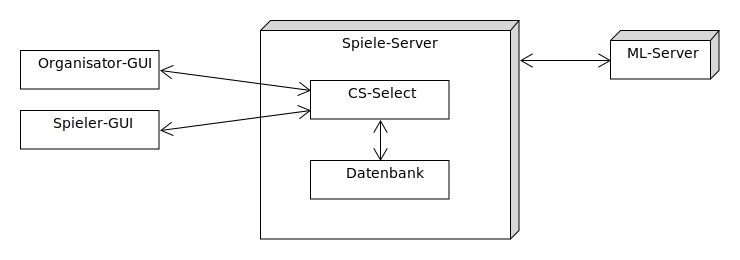
\includegraphics[width=\textwidth]{uml/export/Architektur.png}
    Das Organisator und Spieler GUI läuft in einem Webbrowser. Hier interagieren die Spieler und Organisatoren mit dem \Gls{Produkt}. Der \Gls{Spiele-Server} koordiniert den Spielablauf, speichert Ergebnisse
    in eine Datenbank ab und kommuniziert mit dem ML-Server. Die Kommunikation zwischen Spiele-Server und ML-Server wird durch HTTP-Anfragen stattfinden.
    \section{Anwendungsbereiche}
    Das \Gls{Produkt} dient der Verbesserung der Merkmalsauswahl bei Machine-Learning Prozessen in wissenschaftlichen
    Experimenten beziehungsweise privatwirtschaftlichen Unternehmen durch das Domänenwissen der \Gls{Spieler}.

    \section{Zielgruppen}
    Die Zielgruppen des \Gls{Produkt}s lassen sich in \Glspl{Organisator} und \Glspl{Spieler} unterscheiden.
    Der \Gls{Organisator} möchte eine Verbesserung der Machine-Learning Prozesse erreichen, indem er das Domänenwissen der \Gls{Spieler} nutzt.
    Die \Gls{Spieler} tragen durch Spielen des \Gls{Produkt}s mit ihrem Domänenwissen zur besseren Merkmalsauswahl bei.


    \section{Betriebsbedingungen}
    Das \Gls{Produkt} ist für die Nutzung in Büroräumlichkeiten mit gewöhnlichen Arbeitsplatzrechnern vorgesehen.

    \chapter{Umgebung}
    Das \Gls{Produkt} läuft auf einem Server, die Nutzung erfolgt an Arbeitsplatzrechnern.

    \section{Software}
    Das \Gls{Produkt} läuft auf Linux ab Kernel Version 4 und Windows 7 oder neuer.
    Serverseitig benötigt das Produkt außerdem eine MYSQL-Datenbank, eine Java-Laufzeitumgebung sowie einen verfügbaren Machine-Learning-Server.
    Clientseitig wird entweder Google Chrome oder Mozilla Firefox sowie eine funktionierende Internetverbindung vorausgesetzt.

    \section{Hardware}
    Das \Gls{Produkt} läuft auf Server-Computern, das Frontend wird von gewöhnlichen Arbeitsplatzrechnern angesteuert.

    \section{Machine-Learning-Server}
    Bei dem Machine-Learning-Server handelt es sich um einen Server, der nicht Bestandteil des Produktes ist, jedoch zur Herstellung der Funktionalität benötigt wird.
    Der Machine-Learning-Server kommuniziert mit dem Produkt über das Internet mittels einer REST-API.
    Der Machine-Learning-Server übernimmt das Machine Learning und stellt die Datensätze für das Spiel zur Verfügung.
    Der Machine-Learning-Server unterstützt mindestens die nachfolgenden Anfragen:
    \begin{itemize}
        \item \texttt{GET /features} Liefert einen \Gls{Datensatz} an den Spiel-Server.
        Parameter: Datensatzidentifier
        \item \texttt{GET /score} Bewertet eine Merkmalsauswahl eines \Gls{Spieler}s.
        Gibt eine Zahl zwischen 0 und 1 zurück, die die Güte der Merkmalsauswahl entspricht.
        Parameter: Datensatzidentifier, ausgewählte Merkmale
    \end{itemize}
    
    
    \chapter{Funktionale Anforderungen}
    
    \section{Verwaltung des \Gls{Spiel-Server}s}
    \begin{tabularx}{\linewidth}{@{}>{\bfseries}l@{\hspace{.5em}}X@{}} 
	/F10/ & \Gls{Administrator} konfiguriert eine Config-Datei \\ %Wie schreibt man das am besten
	/F20/ & Globales Passwort für \Glspl{Organisator} muss setzbar sein \\
    \end{tabularx}

    \section{Optional: Einfachere Verwaltung des \Gls{Spiel-Server}s}
    \begin{tabularx}{\linewidth}{@{}>{\bfseries}l@{\hspace{.5em}}X@{}} 
	/F10/ & Bei Start des Systems gibt es ein Dialog zur Einrichtung \\ %Explizit: Was kann man da machen?
	/F20/ & \Glspl{Spiel} sind aus dem System löschbar \\
	/F30/ & Spiel-Server vom Terminal aus beenden \\
	/F40/ & Kontrollierter Neustart: Spiel-Server behält seinen Zustand über Stoppen und Starten hinweg
    \end{tabularx}
    
    \section{Nutzerverwaltung}
    \begin{tabularx}{\linewidth}{@{}>{\bfseries}l@{\hspace{.5em}}X@{}} 
	/F10/ & Erstregistrierung des \Gls{Organisator}s mit E-Mail und global gesetztem Passwort \\ %Machen wir das so?
	/F20/ & Anmelden des \Gls{Organisator}s mit E-Mail und Passwort \\
	/F30/ & Erstregistrierung eines \Gls{Spieler}s mit E-Mail und Passwort, das er in einer Einladungs-E-Mail erhalten hat \\
	/F40/ & Anmelden eines \Gls{Spieler}s mit E-Mail und Passwort \\
    /F50/ & Abmelden der Nutzer
    \end{tabularx}

    \section{Optional: Zusätzliche Funktionen für die Nutzerverwaltung}
    \begin{tabularx}{\linewidth}{@{}>{\bfseries}l@{\hspace{.5em}}X@{}} 
	/F10/ & Änderung der E-Mail \\
	/F20/ & Änderung des Passworts \\
	/F30/ & Zurücksetzen des Passworts ohne Kenntnis des derzeitigen Passworts \\
    \end{tabularx}
    
    \section{Spielerstellung}
    \begin{tabularx}{\linewidth}{@{}>{\bfseries}l@{\hspace{.5em}}X@{}} 
    /F10/ & \Gls{Organisator} kann in Spielerstellungs-GUI \Gls{Spieler} zu einem Spiel einladen, in dem er E-Mail-Adresse angibt \\
    /F20/ & Eingeladene \Gls{Spieler} erhalten Einladungs-E-Mail \\
    /F30/ & \Gls{Organisator} muss mindestens einen \Gls{Spielmodus} auswählen \\
    /F35/ & Falls \Gls{Matrix Select} ausgewählt ist, muss \Gls{Organisator} Matrixgröße angeben \\
    /F50/ & \Gls{Organisator} muss Name des Merkmalsdatensatzes angeben \\
    /F60/ & \Gls{Organisator} muss Adresse einer Datenbank angeben \\ %Kann?
    /F70/ & \Gls{Organisator} muss Spieltitel und Spielbeschreibung angeben \\ %Kann?
    /F80/ & \Gls{Organisator} muss aus den folgenden Möglichkeiten mindestens eine auswählen und gegebenenfalls Werte angeben: Ende nach bestimmter Zeit, Ende nach bestimmter Anzahl an Runden, Ende durch Spielabbruch durch Organisator \\
    /F80/ & \Gls{Organisator} kann Spielerstellung abbrechen \\
    /F90/ & \Gls{Organisator} muss Spielerstellung bestätigen \\
    %Kann Organisator mehrere Spielmodi zur Auswahl für Spieler geben
    \end{tabularx}
    
    \section{Optional: Zusätzliche Funktionen bei der Spielerstellung}
    \begin{tabularx}{\linewidth}{@{}>{\bfseries}l@{\hspace{.5em}}X@{}}
    /F10/ & \Gls{Organisator} kann seine \Gls{Spieleinstellungen} speichern \\
    /F20/ & \Gls{Organisator} kann seine \Gls{Spieleinstellungen} laden \\
    /F30/ & \Gls{Organisator} kann weitere \Gls{Spieler} nach Beginn eines \Gls{Spiel}s einladen \\
    /F40/ & \Gls{Spieler} erhalten über Spieler-GUI eine Benachrichtigung, dass sie eingeladen wurden \\ %Per Mail auch?
	\end{tabularx}
    
    \section{Spielablauf} 
    \begin{tabularx}{\linewidth}{@{}>{\bfseries}l@{\hspace{.5em}}X@{}}
    /F40/ & \Gls{Spieler} kann Einladungen zu Spielen annehmen und ablehnen \\
    /F10/ & \Gls{Spieler} sieht in Spieler-Übersichts-GUI alle Spiele, bei denen er die Einladung angenommen hat und die aktiv sind \\
    /F20/ & \Gls{Spieler} kann Spiel auswählen und spielen, anschließend: \\
    /F30/ & \Gls{Spieler} spielt Runde des entsprechenden \Gls{Spielmodus}, für alle gilt: \\
    /F40/ & \Gls{Spieler} kann Merkmal auswählen \\
    /F40/ & \Gls{Spieler} kann sich zu Merkmal zusätzlich eine Kurzbeschreibung und Grafiken anzeigen lassen \\
    /F40/ & Nach Beenden der Runde sieht der \Gls{Spieler} seine Punktzahl und kann entscheiden, ob er noch eine Runde spielen will \\
	/F50/ & Ein Spiel terminiert nach Erreichen seiner Endbedingungen /Fxxx/, danach kann keine Runde mehr gespielt werden \\
    /F40/ & \Gls{Spieler} sieht in seinem GUI aktuelle Runde und Punktestand \\
	/F60/ & \Gls{Organisator} kann sich über aktuellen Status seines Spiels informieren \\ %Genauer? Gespielte Runden einsehen und so?
	/F70/ & \Gls{Organisator} kann ein Spiel vorzeitig beenden \\
    \end{tabularx}
    
    \subsection{\Gls{Binar Select}}
    \begin{tabularx}{\linewidth}{@{}>{\bfseries}l@{\hspace{.5em}}X@{}}
        /F10/ & Eine Runde Binär Select besteht aus genau fünf Vergleichen \\
    	/F10/ & Dem \Gls{Spieler} werden zufällig immer zwei Merkmale angezeigt \\
    	/F30/ & \Gls{Spieler} muss eines davon auswählen \\
    	/F40/ & \Gls{Spieler} muss bestätigen, dafür muss er genau ein Merkmal ausgewählt haben \\
    \end{tabularx}

    \subsection{\Gls{Matrix Select}}
    \begin{tabularx}{\linewidth}{@{}>{\bfseries}l@{\hspace{.5em}}X@{}}
        /F10/ & Eine Runde Matrix Select besteht aus genau einer Matrix \\
        /F10/ & Es werden zufällige Merkmale in einer Matrix angezeigt \\
    	/F20/ & Genau die Anzahl an Merkmalen, die der \Gls{Organisator} bei Spielerstellung ausgewählt hat, werden angezeigt \\
    	/F30/ & \Gls{Spieler} kann maximal x Merkmale auswählen \\ % Wie viele Merkmale maximal? Gibt es Obergrenze?
    	/F40/ & \Gls{Spieler} muss bestätigen, dafür muss er genau/maximal x Merkmale ausgewählt haben \\ %Wie viele?
    \end{tabularx}
	
	\section{Optional: Zusätzliche Funktionen im Spielablauf}
	\begin{tabularx}{\linewidth}{@{}>{\bfseries}l@{\hspace{.5em}}X@{}} % Linebreaks in der Tabelle
		/F10/ & \Gls{Spieler} kann Runde überspringen, dann: \\
		/F20/ & Von der Gesamtpunktzahl des \Gls{Spieler}s werden 100 Punkte abgezogen, die Gesamtpunktzahl wird aber nicht negativ \\ %100? Kann sie negativ werden?
		/F30/ & \Gls{Spieler} kann ein Merkmal als unwichtig markieren \\
	\end{tabularx}
	
	\section{Optional: Verbesserung der Merkmalsauswahl durch System} 
	\begin{tabularx}{\linewidth}{@{}>{\bfseries}l@{\hspace{.5em}}X@{}} % Linebreaks in der Tabelle
		/F10/ & Die dem \Gls{Spieler} angezeigten Merkmale werden nicht zufällig ausgewählt \\
		/F20/ & Selbe Merkmalskombinationen werden nicht mehrfach in einem Spiel angezeigt \\
	\end{tabularx}
	    
    \section{Bewertung der Merkmalsauswahl des Spielers und Ergebnissicherung}
    \begin{tabularx}{\linewidth}{@{}>{\bfseries}l@{\hspace{.5em}}X@{}} % Linebreaks in der Tabelle
    /F10/ & Merkmalsauswahl des \Gls{Spieler}s wird per http-Anfrage an ML-Server geschickt \\
    /F20/ & Bei \Gls{Matrix Select} wird die ausgewählte Teilmenge der Vergleiche geschickt \\
    /F20/ & Bei \Gls{Binar Select} wird eine gebündelte Menge der Vergleiche geschickt \\
    /F30/ & Rückmeldung wird in Rundenpunktzahl /Fxxx/ umgewandelt \\ %Wie? Das wird bei Punktesystem erklärt
    /F40/ & Rundenpunktzahl wird zur Gesamtpunktzahl des \Gls{Spieler}s addiert \\
    /F50/ & Rundendaten\footnote{Ausgewählte Merkmale, Spielername, Zeitpunkt, Rundenanzahl, Vorhersagequalität, Punkte} werden in von Organisator ausgewählte Datenbank gespeichert \\ %Datenbank zu Spiel
    \end{tabularx}
    
    \section{GUI}
    \begin{tabularx}{\linewidth}{@{}>{\bfseries}l@{\hspace{.5em}}X@{}} % Linebreaks in der Tabelle
    /F10/ & Nutzer haben Zugriff auf die Anmeldungs-GUI in einem Webbrowser \\
    /F20/ & \Glspl{Organisator} erreichen nach erfolgreicher Anmeldung die Organisator-Überschichts-GUI \\
    /F30/ & \Gls{Spieler} erreichen nach erfolgreicher Anmeldung die Spieler-Übersichts-GUI \\
    /F40/ & \Glspl{Organisator} gelangen nach Betätigung der Spielerstellungs-Schaltfläche zur Spielerstellungs-GUI \\
    /F50/ & Nach Beenden der Spielerstellung kehren \Glspl{Organisator} auf die Organisator-Übersichts-GUI zurück \\
    /F60/ & \Gls{Spieler} gelangen nach Betätigung der \enquote{Weiterspielen}-Schaltfläche zur Spiel-GUI \\
    /F70/ & Nach Beenden der Runde kehren \Gls{Spieler} entweder auf die Spieler-Übersichts-GUI oder die Spiel-GUI zurück \\
    /F80/ & Nach Abmeldung kehren Nutzer auf die Anmeldungs-GUI zurück \\
    \end{tabularx}
        
    \section{Gamification-Elemente} %link?
    \label{sec:Gamification-Elemente}
    \begin{tabularx}{\linewidth}{@{}>{\bfseries}l@{\hspace{.5em}}X@{}}
    /F10/ & Punktesystem für \Gls{Spieler} basierend auf ihren Eingaben: \\
    /F15/ & Der für die Merkmalsauswahl erhaltene Wert des \Gls{ML-Server}s wird mit 100 multipliziert und
        auf die nächstgrößere ganze Zahl aufgerundet \\
    \end{tabularx}

    \section{Optional: Weitere Gamification-Elemente}
    \label{sec:Optionale Gamification-Elemente}
    \begin{tabularx}{\linewidth}{@{}>{\bfseries}l@{\hspace{.5em}}X@{}}
	/F10/ & Leaderboard: Auflistung der \Gls{Spieler} mit den meisten Punkten im Spieler-Übersichts-GUI \\
	/F20/ & Achievements: Errungenschaften für \Gls{Spieler}, die freigeschaltet werden können, nachdem der Spieler bestimmte Ziele oder Aufgaben erledigt \\
	/F25/ & Auflistung der Achievements aus /F20/ \\ %in der GUI?
	/F30/ & Daily Challenges: Jeden Tag erhält ein \Gls{Spieler} eine neue Herausforderung, die er abschließen kann \\
	/F40/ & Streaks: Mehr Punkte für einen \Gls{Spieler}, wenn er zwei (oder mehrere) Spiele in Folge spielt \\
	/F50/ & Erweitertes Punktesystem: Abschließen von /Fxx/ und /Fxx/ geben zusätzliche Punkte \\
    \end{tabularx}
    
    \section{Bedienungshilfen}
	\begin{tabularx}{\linewidth}{@{}>{\bfseries}l@{\hspace{.5em}}X@{}}
	/F10/ & Hilfe-Schaltfläche im Organisator-GUI \\ 
	/F20/ & Hilfe Schaltfläche im Spieler-GUI \\ %Die beiden erklären?
	/F30/ & Wenn der Nutzer mit dem Mauszeiger auf einer Schaltfläche im GUI verweilt, erscheint ein Tooltip \\ %Glossar
	\end{tabularx}


    \section{Sprache} %Kapitelname??
    \begin{tabularx}{\linewidth}{@{}>{\bfseries}l@{\hspace{.5em}}X@{}}
	/F10/ & Bereitstellung eines deutschen Sprachpakets für die GUIs \\ 
    \end{tabularx}


    \section{Optional: Internationalisierung}
    \begin{tabularx}{\linewidth}{@{}>{\bfseries}l@{\hspace{.5em}}X@{}}
	/F10/ & Bereitstellung eines englischen Sprachpakets für die GUIs\\
	/F20/ & Änderung der Sprache für Nutzer im GUI möglich \\
    \end{tabularx}

    \section{Optional: Bessere Verfügbarkeit des Systems}
    \begin{tabularx}{\linewidth}{@{}>{\bfseries}l@{\hspace{.5em}}X@{}}
	/F10/ & Unterstützung von Internet Explorer \\
	/F20/ & Unterstützung von Mobilgeräten mit Responsive-GUIs \\
	/F30/ & Lieferung des Servers als Docker-Image \\
	/F40/ & Der Server kann auf verschiedenen Ports ausgeführt werden \\
    \end{tabularx}

    %Kapitel Sonstiges, wenn noch irgendwas einfällt?
    %TODO: Abgeschlossene Spiele löschen

    \chapter{Produktdaten}

    \section{Nutzerdaten}
    \begin{tabularx}{\linewidth}{@{}>{\bfseries}l@{\hspace{.5em}}X@{}}
        /D10/ & Über Nutzer(\Gls{Spieler}, \Gls{Organisator}) sind folgende Daten zu speichern /ND10/: 
        \begin{itemize}
              \item Email-Adresse, Nutzername, Punktestand, Rolle, Passwort(als Hash)
        \end{itemize} \\
        /KD10/ & Über einen \Gls{Spieler} werden außerdem seine Achievements gespeichert. \\
        /KD20/ & Über einen \Gls{Organisator} werden außerdem seine \Gls{Spieleinstellungen} gespeichert. \\
    \end{tabularx}

    \section{Merkmalsdatensätze}
    \begin{tabularx}{\linewidth}{@{}>{\bfseries}l@{\hspace{.5em}}X@{}}
        /D20/ & Für jeden Merkmalsdatensatz ist zu speichern, solange dieser von mindestens einem Spiel benutzt wird: /ND20/: 
        \begin{itemize}
             \item Liste an Merkmalen mit jeweiligen Grafiken und Beschreibung
        \end{itemize}
    \end{tabularx}

    \section{Spieledaten}
    \begin{tabularx}{\linewidth}{@{}>{\bfseries}l@{\hspace{.5em}}X@{}}
        /D30/ & Für jedes \Gls{Spiel} ist zu speichern /ND30/: 
        \begin{itemize}
             \item \Gls{Organisator}, \Gls{Spieleinstellungen}, \Gls{Spieler}, zugehöriger Merkmalsdatensatz, Spielablauf, also Ergebnis einzelner Runden			 % zuständiger ML Server?
			 \item Für jede Runde: Ausgewählte Merkmale, Spielername, Zeitpunkt, Rundenanzahl, Vorhersagequalität, Punkte
		\end{itemize}
    \end{tabularx}


    \chapter{Nichtfunktionale Anforderungen}

    \begin{tabularx}{\linewidth}{@{}>{\bfseries}l@{\hspace{.5em}}X@{}}
        /NF10/ & Es müssen mindestens 30 Spieler zur gleichen Zeit spielen können.\\
        /NF20/ & Die Wartezeiten auf die Reaktion des GUIs dürfen nicht länger als zwei Sekunden betragen. \\
	/NF30/ & Die Anmeldedauer darf nicht mehr als zwei Sekunden betragen. \\
        /NF40/ & Ein Spieler soll das Ergebnis seines Spiels innerhalb von zwei Sekunden erhalten. \\
        /NF50/ & Das Design soll modern wirken. \\
        /NF60/ & Der \Gls{ML-Server} soll leicht austauschbar sein. \\
        /NF70/ & Neue Spielmodi sollen leicht hinzugefügt werden können. \\
        /NF80/ & Neue Spieloberflächen sollen leicht erweiterbar sein. \\
        /NF90/ & Neue Sprachen sollen leicht hinzugefügt werden können. \\
        /NF100/ & Browserkompatibilität: Das Produkt enthält nicht mehr als 0,1\% plattformspezifischer Anweisungen. \\
        /NF110/ & Lizensierung des Produkts mit MIT-Lizenz.
    \end{tabularx}

    \chapter{Testszenarien}
    \section{Organisation}
    \includegraphics[width=\textwidth]{uml/export/Organisation.png}
    Akteure:
    \begin{itemize}
        \item \Gls{Administrator}
        \item \Gls{Organisator}
        \item \Gls{Spieler}
    \end{itemize}
    \newpage
   \subsection{Spieler registrieren}
    \begin{itemize}
        \item Teilnehmende Akteure: \Gls{Organisator}, \Gls{Spieler}
        \item Eingangsaktionen: Spiel-Server ist aktiv
        \item Ereignisfluss:
        \begin{itemize}
            \item \Gls{Organisator} lädt den \Gls{Spieler} über das Organisator-GUI ein.
            \item Der \Gls{Spieler} klickt auf den Einladungslink in der E-Mail und wird auf die Registrierungsseite weitergeleitet.
            \item Der \Gls{Spieler} gibt einen einzigartigen Nutzernamen, seine E-Mail-Adresse sowie ein persönliches Passwort ein und bestätigt.
        \end{itemize}
    \end{itemize}

    \subsection{Spieler anmelden}
    \begin{itemize}
        \item Teilnehmende Akteure: \Gls{Spieler}
        \item Eingangsaktionen: Spiel-Server ist aktiv
        \item Ereignisfluss:
        \begin{itemize}
            \item \Gls{Spieler} öffnet die Produktwebsite
            \item \Gls{Spieler} wählt die Rolle "\Gls{Spieler}" aus
            \item \Gls{Spieler} gibt E-Mail und Passwort ein
            \item \Gls{Spieler} klickt auf anmelden
        \end{itemize}
    \end{itemize}

    \subsection{Spieler löschen}
    \begin{itemize}
        \item Teilnehmende Akteure: \Gls{Administrator}
        \item Eingangsaktionen: Spiele-Server ist aktiv
        \item Ereignisfluss:
        \begin{itemize}
            \item \Gls{Administrator} loggt sich am Server ein
            \item \Gls{Administrator} führt das Löschen-Kommando mit dem Nutzernamen des zu löschenden \Gls{Spieler}s aus
            \item \Gls{Administrator} bestätigt den Vorgang
        \end{itemize}
    \end{itemize}

    \subsection{Organisator registrieren}
    \begin{itemize}
        \item Teilnehmende Akteure: \Gls{Organisator}
        \item Eingangsaktionen: Spiele-Server ist aktiv, Organisator-Registrierungspasswort ist gesetzt
        \item Ereignisfluss:
        \begin{itemize}
            \item \Gls{Organisator} öffnet die Produktwebsite und klickt auf Registrieren
            \item \Gls{Organisator} gibt einen einzigartigen Nutzernamen, seine E-Mail-Adresse, das Organisator-Registrierungspasswort sowie ein persönliches Passwort ein und bestätigt seine Auswahl
        \end{itemize}
    \end{itemize}

    \subsection{Organisator anmelden}
    \begin{itemize}
        \item Teilnehmende Akteure: \Gls{Organisator}
        \item Eingangsaktionen: Spiele-Server ist aktiv
        \item Ereignisfluss:
        \begin{itemize}
            \item \Gls{Organisator} öffnet die Produktwebsite
            \item \Gls{Organisator} wählt die Rolle "\Gls{Organisator}" aus
            \item \Gls{Organisator} gibt E-Mail und Passwort ein
            \item \Gls{Organisator} klickt auf anmelden
        \end{itemize}
    \end{itemize}

    \subsection{Organisator löschen}
    \begin{itemize}
        \item Teilnehmende Akteure: \Gls{Administrator}
        \item Eingangsaktionen: Spiele-Server ist aktiv
        \item Ereignisfluss:
        \begin{itemize}
            \item \Gls{Administrator} loggt sich am Server ein
            \item \Gls{Administrator} führt das Löschen-Kommando mit dem Nutzernamen des zu löschenden \Gls{Organisator}s aus
            \item \Gls{Administrator} bestätigt den Vorgang
        \end{itemize}
    \end{itemize}

    \subsection{Spiel erstellen}
    \begin{itemize}
        \item Teilnehmende Akteure: \Gls{Organisator}, \Gls{Spieler}
        \item Eingangsaktionen: Spiele-Server ist aktiv
        \item Ausgangsaktionen: Spiel starten, \Gls{Spieler} werden eingeladen
        \item Ereignisfluss:
        \begin{itemize}
            \item \Gls{Organisator} meldet sich an
            \item \Gls{Organisator} klickt auf "Spiel erstellen"-Schaltfläche
            \item \Gls{Organisator} sucht sich über seine GUI die gewünschten \Gls{Spieleinstellungen} aus
            \item \Gls{Organisator} lädt \Gls{Spieler} über Angabe der Email in einem Textfeld ein
            \item \Gls{Organisator} bestätigt seine Auswahl und erstellt das Spiel
        \end{itemize}
    \end{itemize}

    \subsection{Spieler nach Spielbeginn einladen}
    \begin{itemize}
        \item Teilnehmende Akteure: \Gls{Organisator}, \Gls{Spieler}
        \item Eingangsaktionen: Spiele-Server ist aktiv, Spiel ist gestartet
        \item Ausgangsaktionen: \Gls{Spieler} werden eingeladen
        \item Ereignisfluss:
        \begin{itemize}
            \item \Gls{Organisator} meldet sich an
            \item \Gls{Organisator} wählt gestartetes Spiel aus der Übersicht
            \item \Gls{Organisator} betätigt "Einladen"-Schaltfläche
            \item \Gls{Organisator} tippt Emails der \Gls{Spieler} in Textfeld ein
            \item \Gls{Organisator} bestätigt seine Auswahl
        \end{itemize}
    \end{itemize}

    \subsection{Spiel vorzeitig beenden}
    \begin{itemize}
        \item Teilnehmende Akteure: \Gls{Organisator}, \Gls{Spieler}
        \item Eingangsaktionen: Spiel ist aktiv und gestartet
        \item Ausgangsaktionen: \Gls{Spieler} können Spiel nicht mehr spielen %werden sie benachrichtigt?
        \item Ereignisfluss:
        \begin{itemize}
            \item \Gls{Organisator} meldet sich an
            \item \Gls{Organisator} wählt gestartetes Spiel aus der Übersicht
            \item \Gls{Organisator} betätigt "Beenden"-Schaltfläche
            \item \Gls{Organisator} bestätigt seine Auswahl
        \end{itemize}
    \end{itemize}

    \subsection{Spiel löschen}
    \begin{itemize}
        \item Teilnehmende Akteure: \Gls{Organisator}
        \item Eingangsaktionen: Spiele-Server ist aktiv, es existiert bereits ein Spiel
        \item Ausgangsaktionen: Spiel löschen
        \item Ereignisfluss:
        \begin{itemize}
            \item \Gls{Organisator} meldet sich an
            \item \Gls{Organisator} wählt über seine GUI das zu löschende Spiel
            \item \Gls{Organisator} bestätigt seine Auswahl
        \end{itemize}
    \end{itemize}

    \subsection{Spieleinstellungen speichern}
    \begin{itemize}
        \item Teilnehmende Akteure: \Gls{Organisator}
        \item Eingangsaktionen: Spiele-Server ist aktiv
        \item Ausgangsaktionen: \Gls{Spieleinstellungen} wiederverwenden
        \item Ereignisfluss:
        \begin{itemize}
            \item \Gls{Organisator} meldet sich an
            \item \Gls{Organisator} sucht sich über seine GUI das Spiel aus, von dem er die Einstellungen speichern möchte
            \item \Gls{Organisator} wählt die Option \enquote{Spieleinstellungen speichern}
            \item \Gls{Organisator} bestätigt seine Auswahl und speichert die Einstellungen
        \end{itemize}
    \end{itemize}

    \subsection{Spieleinstellungen laden}
    \begin{itemize}
        \item Teilnehmende Akteure: \Gls{Organisator}
        \item Eingangsaktionen: Spiele-Server ist aktiv, \Gls{Spieleinstellungen} wurden bereits gespeichert
        \item Ausgangsaktionen: Spiel starten
        \item Ereignisfluss:
        \begin{itemize}
            \item \Gls{Organisator} meldet sich an
            \item \Gls{Organisator} erstellt über seine GUI ein neues Spiel
            \item \Gls{Organisator} wählt für dieses Spiel \enquote{Spieleinstellungen laden}
            \item \Gls{Organisator} sucht sich die bereits gespeicherte \Gls{Spieleinstellungen} heraus
            \item \Gls{Organisator} bestätigt seine Auswahl
        \end{itemize}
    \end{itemize}

    \subsection{Ergebnisse auslesen}

    \begin{itemize}
        \item Teilnehmende Akteure: \Gls{Organisator}
        \item Eingangsaktionen: \Gls{Organisator} öffnet die Auswertungsseite
        \item Ausgangsaktionen: \Gls{Organisator} erhält die Auswertung
        \item Ereignisfluss -
    \end{itemize}
 \subsection{Spielzustand auslesen}
	\begin{itemize}
		\item Teilnehmende Akteure: \Gls{Organisator}
		\item Eingangsaktionen: Spiele-Server ist aktiv
		\item Ereignisfluss:
		\begin{itemize}
			\item \Gls{Organisator} meldet sich an
			\item \Gls{Organisator} erreicht seine Übersichtsseite
			\item \Gls{Organisator} sieht den Zustand seiner laufenden Spiele
		\end{itemize}
	\end{itemize}


    \newpage
    \section{Spiel}
    \includegraphics[width=\textwidth]{uml/export/Spiel.png}
    Akteure: 
    \begin{itemize}
    \item \Gls{Spieler}
    \newpage
    \end{itemize}
    
   
    \subsection{Runde spielen: Matrix Select}
    \begin{itemize}
    	\item Teilnehmende Akteure: \Gls{Spieler}
    	\item Eingangsaktionen: Spiele-Server ist aktiv, Spieler hat offenes Spiel des \Gls{Spielmodus} Matrix Select
    	\item Ereignisfluss:
    	\begin{itemize}
    		\item \Gls{Spieler} meldet sich an
    		\item \Gls{Spieler} erreicht seine Übersichtsseite
    		\item \Gls{Spieler} klickt auf Weiterspielen-Schaltfläche
    		\item \Gls{Spieler} erreicht Spiel-GUI
    		\item \Gls{Spieler} klickt auf ein Merkmal und sieht Merkmalsgraphen und Merkmalsbeschreibung
    		\item \Gls{Spieler} wählt mehrere Merkmale aus
    		\item \Gls{Spieler} klickt auf Schaltfläche, um Auswahl zu bestätigen
    	\end{itemize}
    \end{itemize}
	
	\subsection{Runde spielen: Binär Select}
	\begin{itemize}
		\item Teilnehmende Akteure: \Gls{Spieler}
		\item Eingangsaktionen: Spiele-Server ist aktiv, \Gls{Spieler} hat offenes Spiel des \Gls{Spielmodus} Binär Select
		\item Ereignisfluss:
		\begin{itemize}
			\item \Gls{Spieler} meldet sich an
			\item \Gls{Spieler} erreicht seine Übersichtsseite
			\item \Gls{Spieler} klickt auf Weiterspielen-Schaltfläche
			\item \Gls{Spieler} erreicht Spiel-GUI
			\item \Gls{Spieler} klickt auf ein Merkmal und sieht Merkmalsgraphen und Merkmalsbeschreibung
			\item \Gls{Spieler} wählt eines der beiden Merkmale aus
			\item \Gls{Spieler} klickt auf Schaltfläche, um Auswahl zu bestätigen
		\end{itemize}
	\end{itemize}

	\subsection{Auswahl überspringen}
	\begin{itemize}
		\item Teilnehmende Akteure: \Gls{Spieler}
		\item Eingangsaktionen: Spiele-Server ist aktiv, \Gls{Spieler} hat offenes Spiel
        \item Ausgangsaktionen: Der \Gls{Spieler} kommt in die nächste Runde des aktiven Spiels
		\item Ereignisfluss:
		\begin{itemize}
			\item \Gls{Spieler} meldet sich an
			\item \Gls{Spieler} erreicht seine Übersichtsseite
			\item \Gls{Spieler} klickt auf Weiterspielen-Schaltfläche
			\item \Gls{Spieler} erreicht Spiel-GUI
			\item \Gls{Spieler} klickt Auswahl-Überspringen-Schaltfläche und bestätigt seine Auswahl
            \item Dem \Gls{Spieler} werden Punkte abgezogen
		\end{itemize}
	\end{itemize}
     
    \subsection{Streak erreichen}\footnote{Zur Erklärung von Streak siehe \fref{fig:Streak_State}}
    \begin{itemize}
        \item Teilnehmende Akteure: \Gls{Spieler}
        \item Eingangsaktionen: \Gls{Spieler} spielt eine Runde
        \item Ausgangsaktionen: \Gls{Spieler} erhält extra Punkte für seine Runde
        \item Ereignisfluss:
        \begin{itemize}
            \item \Gls{Spieler} spielt n Runden um eine Streak zu erreichen.
            \item System teilt dem \Gls{Spieler} mit, dass er eine Streak erreicht hat.
        \end{itemize}
    \end{itemize}
    
\newpage
    \section{Spieler-Übersicht}
    \includegraphics[width=\textwidth]{uml/export/Spieler_Ubersicht.png}
	    \subsection{Achievements ansehen}
    \begin{itemize}
        \item Teilnehmende Akteure: \Gls{Spieler}
        \item Eingangsaktionen: Spiele-Server ist aktiv
        %\item Ausgangsaktionen: Achievements ansehen
        \item Ereignisfluss:
        \begin{itemize}
            \item \Gls{Spieler} meldet sich an
            \item \Gls{Spieler} erreicht seine Übersicht-Seite
            \item \Gls{Spieler} klickt auf die Spieler-Übersicht-Schaltfläche
            \item \Gls{Spieler} schaut seine Achievements an
        \end{itemize}
    \end{itemize}
    %Nach der Anmeldung erreicht ein \Gls{Spieler} eine Übersichts-Seite. Beim Klicken auf die Spieler-Übersicht-Schaltfläche
    %(in \fref{fig:Spieler-Übersicht} gezeigt) kann der \Gls{Spieler} seine \Gls{Achievement}s einsehen.
    \subsection{Leaderboard ansehen}
    \begin{itemize}
        \item Teilnehmende Akteure: \Gls{Spieler}
        \item Eingangsaktionen: Spiele-Server ist aktiv
        %\item Ausgangsaktionen: Leaderboard ansehen
        \item Ereignisfluss:
        \begin{itemize}
            \item \Gls{Spieler} meldet sich an
            \item \Gls{Spieler} erreicht seine Übersichtsseite
            \item \Gls{Spieler} sieht dort in einer Tabelle die \Gls{Spieler} mit den meisten Punkten über einen gewissen Zeitraum
        \end{itemize}
    \end{itemize}
    %Nach der Anmeldung erreicht ein \Gls{Spieler} eine Übersichts-Seite. Darauf ist ein Bereich, der eine aktuelle Tabelle
    %anzeigt, in welcher die \Gls{Spieler} aufgelistet sind, die in einem bestimmten Zeitraum die meisten Punkte erreicht haben.
    \newpage
    \section{Administration}
    \includegraphics[width=\textwidth]{uml/export/Administration.png}
     \subsection{Sprache ändern}
    \begin{itemize}
    \item Teilnehmende Akteure: \Gls{Spieler}, \Gls{Organisator}
    \item Eingangsaktionen: Spiele-Server ist aktiv
    \item Ereignisfluss:
        \begin{itemize}
            \item \Gls{Organisator} oder \Gls{Spieler} meldet sich an
            \item \Gls{Organisator} oder \Gls{Spieler} erreicht seine Übersichtsseite
            \item \Gls{Organisator} oder \Gls{Spieler} wählt die Sprachänderungs-Schaltfläche aus
            \item \Gls{Organisator} oder \Gls{Spieler} bestätigt seine Auswahl
        \end{itemize}
    \end{itemize}
    \subsection{Server installieren}
    \begin{itemize}
        \item Teilnehmende Akteure: \Gls{Administrator} 
        \item Eingangsaktionen: Computer mit MySQL und Tomcat installiert
        \item Ausgangsaktionen: Spiele-Server starten
        \item Ereignisfluss: 
            \begin{itemize}
                \item \Gls{Administrator} kopiert die War Datei in den Tomcat webapps Ordner
                \item \Gls{Administrator} fügt den Pfad zur CFG Datei in die `tomcat/conf/Catalina/<host>` Datei ein
                \item \Gls{Administrator} konfiguriert die CFG Datei aus der Dokumentation mit den relevanten Werten
                \item \Gls{Administrator} führt \texttt{tomcat/bin/startup.sh}(Linux \& Mac) bzw. \texttt{tomcat\textbackslash bin\textbackslash startup.bat}(Windows) aus
            \end{itemize}
    \end{itemize}

    \subsection{Server beenden}
    \begin{itemize}
        \item Teilnehmende Akteure: \Gls{Administrator}
        \item Eingangsaktionen: Spiele-Server ist aktiv
        \item Ausgangsaktionen: MySQL beenden, falls sonst nichts Weiteres auf der Datenbank läuft
        \item Ereignisfluss: \Gls{Administrator} führt \texttt{tomcat/bin/shutdown.sh}(Linux \& Mac) bzw. \texttt{tomcat\textbackslash bin\textbackslash shutdown.bat}(Windows)
    \end{itemize}

    \subsection{Punkte eines Spielers zurücksetzen}
    \begin{itemize}
        \item Teilnehmende Akteure: \Gls{Administrator}, \Gls{Spieler}
        \item Eingangsaktionen: Spiele-Server ist aktiv
        \item Ausgangsaktionen: Die Punkte des \Gls{Spieler}s sind zurückgesetzt
        \item Ereignisfluss:
        \begin{itemize}
            \item \Gls{Administrator} loggt sich in Spiele-Server ein
            \item \Gls{Administrator} gibt das "Punkte zurücksetzen"-Kommando und die Email des registrierten Spielers ein
            \item \Gls{Administrator} bestätigt seine Auswahl
            \item Die Punkte des entsprechenden \Gls{Spieler}s werden zurückgesetzt
        \end{itemize}
    \end{itemize}




    \subsection{Passwort ändern}
    \begin{itemize}
    \item Teilnehmende Akteure: \Gls{Spieler}, \Gls{Organisator}
    \item Eingangsaktionen: Spiele-Server ist aktiv
    \item Ereignisfluss:
        \begin{itemize}
            \item \Gls{Organisator} oder \Gls{Spieler} meldet sich an
            \item \Gls{Organisator} oder \Gls{Spieler} erreicht seine Übersichtsseite
            \item \Gls{Organisator} oder \Gls{Spieler} wählt die Profileinstellungen aus
            \item \Gls{Organisator} oder \Gls{Spieler} klickt aus die \enquote{Passwort ändern}-Schaltfläche
            \item \Gls{Organisator} oder \Gls{Spieler} gibt sein aktuelle sowie sein neues gewünschtes Passwort ein
            \item \Gls{Organisator} oder \Gls{Spieler} bestätigt seine Auswahl
        \end{itemize}
    \end{itemize}

    \subsection{Passwort zurücksetzen}
    \begin{itemize}
        \item Teilnehmende Akteure: \Gls{Spieler}, \Gls{Organisator}
        \item Eingangsaktionen: Spiele-Server ist aktiv
        \item Ausgangsaktionen: Temporäres Passwort ändern
        \item Ereignisfluss:
        \begin{itemize}
            \item \Gls{Organisator} oder \Gls{Spieler} öffnet die Produktwebsite und klickt auf \enquote{Passwort zurücksetzen}
            \item \Gls{Organisator} oder \Gls{Spieler} erhält per Mail ein neues temporäres Passwort
            \item \Gls{Organisator} oder \Gls{Spieler} meldet sich mit dem neuen Passwort an
        \end{itemize}
    \end{itemize}
       \subsection{Hilfe-Schaltfläche verwenden}
    \begin{itemize}
        \item Teilnehmende Akteure: \Gls{Spieler}, \Gls{Organisator}
        \item Eingangsaktionen: \Gls{Spieler} oder \Gls{Organisator} benötigt Hilfe mit dem Produkt
        \item Ausgangsaktionen: System zeigt dem Akteur die relevante Hilfe Seite
        \item Ereignisfluss:
            \begin{itemize}
                \item \Gls{Spieler} oder \Gls{Organisator} klickt auf die Hilfe-Schaltfläche(oben links)
            \end{itemize}
    \end{itemize}

    %TODO: Ausführung auf verschiedenem Ports

    \chapter{Dynamische Modelle}
    \section{Zustandsdiagramme}
    \subsection{Streak}
    \label{fig:Streak_State}
    
\includegraphics[width=\textwidth]{uml/export/Streak_Zustand.png}
    Die Zustände, die eine Streak haben kann. Eine Streak ist immer auf einen Spieler beschränkt.
    Zustandbeschreibung:
    \begin{itemize}
    \item begonnen: Eine angefangene Steak, die noch nicht lang genug ist, um für den Spieler eine erhöhte Punktzahl zu erreichten.
    \item aktiv: Die Streak ist lang genug. In diesem Zustand erhält der Spieler Punkte * Faktor Punkte. (Faktor $\geq$ 1)
    \end{itemize}
    \subsection{Spiel}
    \label{fig:Spiel_State}
    
\includegraphics[width=\textwidth]{uml/export/Spiel_Zustand.png}
    Die Zustände, die ein Spiel von der Erstellung bis zum beenden haben kann.
    Zustandsbeschreibung:
    \begin{itemize}
    \item existiert: Das Spiel existiert, besitzt also einen Datensatz, Endbedingungen und Spielmodus. Es sind aber noch keine Spieler eingeladen, also kann es nicht gespielt werden.
    \item läuft: Das Spiel kann von Spielern gespielt werden.
    \item beendet: Das Spiel wurde beendet. Kein Spieler kann mehr eine Runde spielen. Die Ergebnisse können aber noch ausgelesen werden. 
    \end{itemize}
    \subsection{Achievements}
    \label{fig:Achievment_State}
    
\includegraphics[width=\textwidth]{uml/export/Achievment_State.png}
    Die Zustände die ein Achievment von \enquote{Spieler kennt das Achievment nicht} bis zu \enquote{Spieler hat das Achievment erreicht}.
    \begin{itemize}
    \item Nicht sichtbar: Spieler weiß nicht, dass das Achievment existiert.
    \item Verdeckt: Spieler weiß, dass dieses Achievment existiert, aber nicht was er tun muss um es zu erreichen.
    \item Freigeschaltet: Die Bedingungen für das Erreichen dieses Achievments sind dem Spieler bekannt.
    \item Erreicht: Der Spieler hat die Bedingungen für das Erreichen dieses Achievments erfüllt.
    \end{itemize}
    

    \chapter{Benutzerschnittstelle}

    \section{Anmeldung}
    \centering
    \includegraphics[width=\textwidth]{../pictures/Anmeldung.jpg}
    \subsection{Anmeldung (responsive)}
    \centering
    \includegraphics[width=\textwidth]{../pictures/Anmeldung_responsive.jpg}

    \section{Organisator-Start}
    \centering
    \includegraphics[width=\textwidth]{../pictures/2_Organisator.jpg}

    \subsection{Organisator-Start (responsive)}
    \centering
    \includegraphics[width=\textwidth]{../pictures/3_Organisator(responsive).jpg}
    In den weiteren Darstellungen werden keine responsiven Darstellungen gezeigt, die zwei bereits gezeigten Darstellungen dienen als anschauliches Beispiel für
    responsive Darstellung einer Benutzerschnittstelle.

    \section{Spielerstellung}
    \centering
    \includegraphics[width=\textwidth]{../pictures/Spielerstellung.jpg}

    \section{Spieler-Übersicht}
    \label{fig:Spieler-Übersicht}
    \centering
    \includegraphics[width=\textwidth]{../pictures/5_Spieler.jpg}

    \section{Spiel}
    \subsection{Matrix Select}
    \centering
    \includegraphics[width=\textwidth]{../pictures/MatrixSelect.jpg}
    \subsection{Binär Select}
    \centering
    \includegraphics[width=\textwidth]{../pictures/BinSelect.jpg}

    \clearpage


    \chapter{Glossar}
    \printglossary
    
\end{document}
